\documentclass[10pt, xcolor=table]{beamer}
\usetheme{metropolis}
% all imports
\usepackage[utf8]{inputenc}
\usepackage[T1]{fontenc}
\usepackage{lmodern}
\usepackage{appendixnumberbeamer}
\usepackage{hyperref}
\usepackage{booktabs}
\usepackage{bm}
\usepackage[scale=2]{ccicons}
\usepackage[outputdir=build]{minted}
\usepackage{pgfplots}
\usepackage{array,colortbl,xcolor}
\usepgfplotslibrary{dateplot}
\usepackage{setspace}
\usepackage{etoolbox}
\usepackage{xspace}
\usepackage{tikz}
\usetikzlibrary{shapes,arrows,positioning,fit,backgrounds}
\usepackage{tkz-euclide}
\usepackage{soul}
\usepackage{ragged2e}
\usepackage{algorithm}
\usepackage[noend]{algpseudocode}
\usepackage{caption}
\usepackage{amsmath}
\def\HiLi{\leavevmode\rlap{\hbox to \hsize{\color{yellow!50}\leaders\hrule height .8\baselineskip depth .5ex\hfill}}}
\title{Presentation_RRT_AP}

\AtBeginEnvironment{quote}{\singlespacing}

% new commands
\newcommand{\themename}{\textbf{\textsc{metropolis}}\xspace}
\newcommand{\vect}[1]{\bm{#1}}
\newcommand{\myprime}[1]{{#1}^{\prime}}
\newcommand{\grad}[2]{\nabla_{#1} {#2}}
\newcommand{\dotp}[2]{{#1}^{\top}{#2}}
\newcommand{\dotpPright}[2]{{#1}^{\top}\left({#2}\right)}
\newcommand{\outerp}[2]{\left({#1}\right){#2}^{\top}}
\newcommand{\Jacobian}[2]{\frac{\partial #1}{\partial #2}}
\newcommand{\Vocab}{\mathbb{V}}
\DeclareMathOperator*{\argmin}{arg\,min}

% Quote with author reference at the end
\let\oldquote\quote
\let\endoldquote\endquote
\renewenvironment{quote}[2][]
  {\if\relax\detokenize{#1}\relax
     \def\quoteauthor{#2}%
   \else
     \def\quoteauthor{#2~---~#1}%
   \fi
   \oldquote}
  {\par\nobreak\smallskip\hfill(\quoteauthor)%
   \endoldquote\addvspace{\bigskipamount}}
%-----------------------------------------   
% Justifying itemize
% \let\olditem\item
% \renewcommand\item{\olditem\justifying}
%----------------------------------------- 
% Change default caption of algorithm environment
\DeclareCaptionFormat{myformat}{#3}
\captionsetup[algorithm]{format=myformat}
%----------------------------------------- 
% Enables line numbering in any order
\newcommand{\setalglineno}[1]{%
  \setcounter{ALG@line}{\numexpr#1-1}}
  
\algnewcommand\And{\textbf{AND}}
\algnewcommand\Or{\textbf{OR}}
\renewcommand{\algorithmicloop}{\textbf{forever}}

\newlength\myindent
\setlength\myindent{2em}
\newcommand\bindent{%
  \begingroup
  \setlength{\itemindent}{\myindent}
  \addtolength{\algorithmicindent}{\myindent}
}
\newcommand\eindent{\endgroup}

% definitions 
\definecolor{blue}{RGB}{159, 192, 176}
\definecolor{green}{RGB}{160, 227, 127}
\definecolor{orange}{RGB}{243, 188, 125}
\definecolor{red}{RGB}{253, 123, 84}
\definecolor{nephritis}{RGB}{39, 174, 96}
\definecolor{emerald}{RGB}{46, 204, 113}
\definecolor{turquoise}{RGB}{39, 174, 96}
\definecolor{green-sea}{RGB}{22, 160, 133}
% Tikzstyles for Computation Graphs

% nodes
\tikzstyle{noop} = [circle, draw=none, fill=red, minimum size = 10pt]
\tikzstyle{op} = [circle, draw=red, line width=1.5pt, fill=red!70, text=black, text centered, font=\bf \normalsize, minimum size = 25pt]
\tikzstyle{state} = [circle, draw=blue, line width=1.5pt, fill=blue!70, text=black, text centered, font=\bf \normalsize, minimum size = 25pt]
% \tikzstyle{gradient} = [circle, draw=green, line width=1.5pt, fill=green!60, text=black, text centered, font=\bf \normalsize, minimum size = 25pt]
\tikzstyle{gradient} = [circle, draw=nephritis, line width=1.5pt, fill=nephritis!60, text=black, text centered, font=\bf \normalsize, minimum size = 25pt]
\tikzstyle{textonly} = [draw=none, fill=none, text centered, font=\bf \normalsize]
\tikzstyle{boxtextonly} = [draw=none, fill=none, align=center, font=\bf \normalsize]

% edges
% \tikzstyle{tedge}  = [draw, thick, >=stealth, ->]
\tikzstyle{tedge}  = [draw, thick, >=latex, ->]

% namedscope
\tikzstyle{namedscope} = [circle, draw=orange, line width=1.5pt, fill=orange!60, align=center, inner sep=0pt]

% \tikzstyle{container} = [draw=none, rectangle, dotted, inner ysep=1.5em]
% \tikzstyle{novertex} = [draw=none, fill=none, text centered]
% \tikzstyle{predicate} = [ellipse, draw, thick, text centered, rounded corners, minimum size=30pt]
% \tikzstyle{aux} = [rectangle, draw, thick, text centered, rounded corners, minimum size=30pt]
% \tikzstyle{ledge}  = [draw, dashed, thick, >=stealth, ->]
% \tikzstyle{pedge}  = [draw, thick, >=stealth, ->]



\title{Rapidly-Exploring Random Trees: \\
\Large from an automated planning perspective} 
\date{\today}
\author{Paula Moraes}
\institute{\textbf{IME-USP}: Institute of Mathematics and Statistics - University of Sao Paulo}

\titlegraphic{
            \hspace{9cm}
            
\includegraphics[scale=0.2]{images/logo0red.png}
}



\begin{document}

\graphicspath{ {images/} }

\maketitle

\section{Revision Motion Planning}

\begin{frame}{Motion Planning}
\justify
Motion Planning is an important area in \alert{robotics} that addresses the problem of finding a sequence of control inputs so as to drive the robot from its initial state (or configuration) to one of the goal states while \alert{obeying the rules of the environment} \cite{karaman2011sampling} \\

This problem is known to be at least PSPACE-hard... % achar referencia e colocar

Besides robotics other areas rely on motion planning algorithms:
\begin{itemize}
\item computer graphics
\item computational biology
\item virtual prototyping
\end{itemize}
\end{frame}

\begin{frame}{Configuration Space - $C_{space}$}
$C_{space}$ is the space of all possible configurations (or positions) that a system can attain given its rigid body degrees of freedom (DOF\footnote[frame]{the number of independent parameters that define its configuration}) and the presence of obstacles in the environment. 

\hspace{1cm}
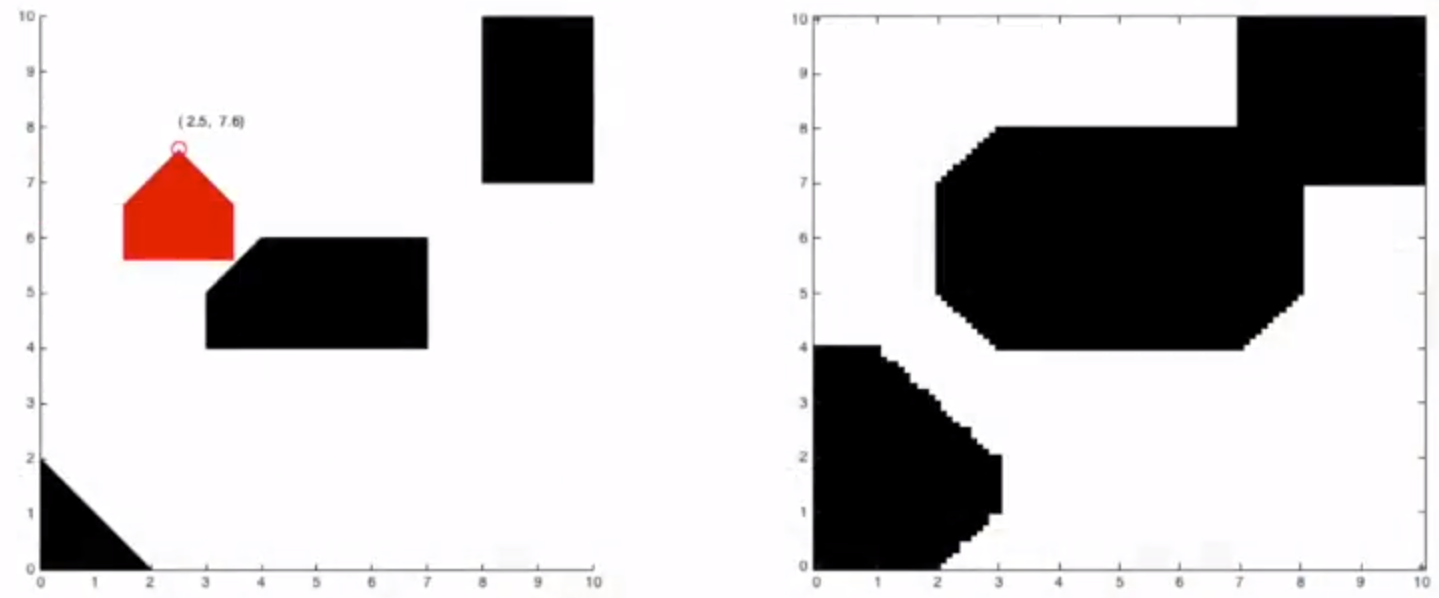
\includegraphics[width=10cm,height=5cm]{cspace.png} 

\end{frame}

\begin{frame}{The need of sampling-based methods}
Since real world applications often requires planning in high-dimensional spaces, an \alert{explicit representation} of the obstacles in $C_{space}$ to construct a solution is \alert{unfeasible}. 

Introduced in the mid-90s, \textbf{sampling-based algorithms} avoided representations of the world by relying on a \alert{collision checking module} building a graph with only the feasible trajectories.

\begin{itemize}
\item \textit{Probabilistic RoadMaps} - constructs a graph of sets of collision-free trajectories to then answer multiple queries by computing a shortest path that connects the initial with a final state through the roadmap \cite{karaman2011sampling}
\item \textit{Rapidly-Exploring Random Trees} - incrementally grows a tree from an initial configuration towards unexplored portions of the space until the goal region is reached 
\end{itemize}

\end{frame}

\section{Rapidly-Exploring Random Trees}

\begin{frame}{Overview}
RRT is an efficent \alert{data structure} and \alert{sampling scheme} to quickly search high-dimensional spaces \cite{lavalle2000rapidly}, widely used in \alert{continuous} path planning problems. 

The exploration is biased toward unexplored regions by sampling random points and incrementally growing the search tree towards them.

Caracteristics:
\begin{itemize}
\item suboptimal 
\item probabilistic completeness
\item aimed at single-query applications
\item heavily relies on a collision checking module given it doesn't explicit construct obstacles in the state space
\end{itemize}
\end{frame}

\begin{frame}{Step-by-step basic RRT algorithm}
\begin{algorithm}[H]
\caption{BUILD\_RRT($q_{\text{init}}$)}
\begin{algorithmic}[1]
\State \textit{tree} $\gets$ $q_{\text{init}}$;
\While{$\neg$\textit{end\_criteria}} 
  \State \HiLi$q_{\text{rand}} \gets$ RANDOM\_STATE();
  \State EXTEND($q_{\text{rand}}$, \textit{tree});
\EndWhile
\State return \textit{tree};
\end{algorithmic}
\end{algorithm}
\vspace{-0.6cm}
\begin{algorithm}[H]
\caption{EXTEND($q_{\text{rand}}$, \textit{tree})}
\begin{algorithmic}[1]
\State $q_{\text{near}}$ $\gets$ NEAREST\_NEIGHBOR($q_{\text{rand}}$, \textit{tree});
\State ($q_{\text{new}}$, \textit{collided}) $\gets$ NEW\_STATE($q_{\text{rand}}$, $q_{\text{near}}$, FIXED\_STEP\_SIZE, SEARCH\_SPACE);
\If{$\neg$\textit{collided}}
  \State add\_vertex($q_{\text{new}}$, \textit{tree});
  \State add\_edge($q_{\text{new}}$, $q_{\text{near}}$,\textit{tree});
  \If{$q_{\text{new}} = q_{\text{rand}}$}
    \State return \textit{Reached};
  \Else
    \State return \textit{Advanced};  
  \EndIf
\EndIf 
\State return \textit{Trapped};
\end{algorithmic}
\end{algorithm}
% \begin{algorithm}[H]
% \caption{BUILD\_RRT($q_{\text{init}}$)}
% \begin{algorithmic}[1]
% \State \textit{tree} $\gets$ $q_{\text{init}}$;
% \While{$\neg$\textit{end\_criteria}} 
%   \State $q_{\text{rand}} \gets$ RANDOM\_STATE();
% \EndWhile
% \end{algorithmic}
% \end{algorithm}
\end{frame}

\begin{frame}{Sampling random state}
\begin{tikzpicture}[scale=1.5]
\draw [fill=black!30!green] (0,0) circle [radius =0.1] -- (0.8,-0.2) circle [radius =0.1];
\draw [fill=black!30!green] (0,0) circle [radius =0.1] -- (-0.5,0.5) circle [radius =0.1];
\node [] at (0,-0.3) {$q_{\text{init}}$};
\draw [fill=black!30!green] (-0.5,0.5) circle [radius =0.1] -- (-1.3,0.5) circle [radius =0.1];
\draw [fill=black!30!green] (0.8,-0.2) circle [radius =0.1] -- (1.4,0.3) circle [radius =0.1];
\draw [fill=black!30!green] (0.8,-0.2) circle [radius =0.1] -- (1.4,-0.6) circle [radius =0.1];
\draw [fill=black!30!green] (1.4,0.3) circle [radius =0.1] -- (2,0.3) circle [radius =0.1]; % criar no a partir dele para começar a explicar

\draw [fill=black!30!green] (2,0.3) circle [radius =0.1] -- (2.6,0.1) circle [radius =0.1]; % q_near
% \node [] at (2.6,-0.2) {$q_{\text{near}}$};
\draw [fill=black!30!green] (5.6,1.5) circle [radius =0.1]; 
\node [] at (5.6,1.2) {$q_{\text{rand}}$};

\end{tikzpicture}

\vspace{1cm}
\captionof{figure}{Tree rooted at $q_{init}$ and sampled state $q_{rand}$}
\vspace{0.3cm}
% \textit{Sampling: $q_{\text{rand}} \to \textit{U}(C_\text{space})$}
\alert{\textit{Sampling: $\textit{U}(C_\text{space}) \to q_{\text{rand}}$}}
\end{frame}

\begin{frame}{Step-by-step basic RRT algorithm}
\vspace{-0.2cm}
\begin{algorithm}[H]
\caption{BUILD\_RRT($q_{\text{init}}$)}
\begin{algorithmic}[1]
\State \textit{tree} $\gets$ $q_{\text{init}}$;
\While{$\neg$\textit{end\_criteria}} 
  \State $q_{\text{rand}} \gets$ RANDOM\_STATE();
  \State EXTEND($q_{\text{rand}}$, \textit{tree});
\EndWhile
\State return \textit{tree};
\end{algorithmic}
\end{algorithm}
\vspace{-0.6cm}
\begin{algorithm}[H]
\caption{EXTEND($q_{\text{rand}}$, \textit{tree})}
\begin{algorithmic}[1]
\State \HiLi$q_{\text{near}}$ $\gets$ NEAREST\_NEIGHBOR($q_{\text{rand}}$, \textit{tree});
\State ($q_{\text{new}}$, \textit{collided}) $\gets$ NEW\_STATE($q_{\text{rand}}$, $q_{\text{near}}$, FIXED\_STEP\_SIZE, SEARCH\_SPACE);
\If{$\neg$\textit{collided}}
  \State add\_vertex($q_{\text{new}}$, \textit{tree});
  \State add\_edge($q_{\text{new}}$, $q_{\text{near}}$,\textit{tree});
  \If{$q_{\text{new}} = q_{\text{rand}}$}
    \State return \textit{Reached};
  \Else
    \State return \textit{Advanced};  
  \EndIf
\EndIf 
\State return \textit{Trapped};
\end{algorithmic}
\end{algorithm}
% \begin{algorithm}[H]
% \caption{BUILD\_RRT($q_{\text{init}}$)}
% \begin{algorithmic}[1]
% \State \textit{tree} $\gets$ $q_{\text{init}}$;
% \While{$\neg$\textit{end\_criteria}} 
%   \State $q_{\text{rand}} \gets$ RANDOM\_STATE();
%   \State EXTEND($q_{\text{rand}}$, \textit{tree});
% \EndWhile
% \end{algorithmic}
% \end{algorithm}
% \vspace{-0.6cm}
% \begin{algorithm}[H]
% \caption{EXTEND($q_{\text{rand}}$, \textit{tree})}
% \begin{algorithmic}[1]
% \State $q_{\text{near}}$ $\gets$ NEAREST\_NEIGHBOR($q_{\text{rand}}$, \textit{tree});
% \end{algorithmic}
% \end{algorithm}
\end{frame}

\begin{frame}{Finding nearest neighbor}
\begin{tikzpicture}[scale=1.5]
\draw [fill=black!30!green] (0,0) circle [radius =0.1] -- (0.8,-0.2) circle [radius =0.1];
\draw [fill=black!30!green] (0,0) circle [radius =0.1] -- (-0.5,0.5) circle [radius =0.1];
\node [] at (0,-0.3) {$q_{\text{init}}$};
\draw [fill=black!30!green] (-0.5,0.5) circle [radius =0.1] -- (-1.3,0.5) circle [radius =0.1];
\draw [fill=black!30!green] (0.8,-0.2) circle [radius =0.1] -- (1.4,0.3) circle [radius =0.1];
\draw [fill=black!30!green] (0.8,-0.2) circle [radius =0.1] -- (1.4,-0.6) circle [radius =0.1];
\draw [fill=black!30!green] (1.4,0.3) circle [radius =0.1] -- (2,0.3) circle [radius =0.1]; % criar no a partir dele para começar a explicar

\draw [fill=black!30!green] (2,0.3) circle [radius =0.1] -- (2.6,0.1) circle [radius =0.1]; % q_near
\node [] at (2.6,-0.2) {$q_{\text{near}}$};
\draw [fill=black!30!green, dashed] (2.6,0.1) circle [radius =0.1] -- (5.6,1.5) circle [radius =0.1]; 
\node [] at (5.6,1.2) {$q_{\text{rand}}$};

\end{tikzpicture}

\vspace{1cm}
\captionof{figure}{$q_{near}$ is the closest state to $q_{rand}$ that already belongs to the tree}
\end{frame}

\begin{frame}{Step-by-step basic RRT algorithm}
\vspace{-0.2cm}
\begin{algorithm}[H]
\caption{BUILD\_RRT($q_{\text{init}}$)}
\begin{algorithmic}[1]
\State \textit{tree} $\gets$ $q_{\text{init}}$;
\While{$\neg$\textit{end\_criteria}} 
  \State $q_{\text{rand}} \gets$ RANDOM\_STATE();
  \State EXTEND($q_{\text{rand}}$, \textit{tree});
\EndWhile
\State return \textit{tree};
\end{algorithmic}
\end{algorithm}
\vspace{-0.6cm}
\begin{algorithm}[H]
\caption{EXTEND($q_{\text{rand}}$, \textit{tree})}
\begin{algorithmic}[1]
\State $q_{\text{near}}$ $\gets$ NEAREST\_NEIGHBOR($q_{\text{rand}}$, \textit{tree});
\State \HiLi($q_{\text{new}}$, \textit{collided}) $\gets$ NEW\_STATE($q_{\text{rand}}$, $q_{\text{near}}$, FIXED\_STEP\_SIZE, \
       \HiLi SEARCH\_SPACE);
\If{$\neg$\textit{collided}}
  \State add\_vertex($q_{\text{new}}$, \textit{tree});
  \State add\_edge($q_{\text{new}}$, $q_{\text{near}}$,\textit{tree});
  \If{$q_{\text{new}} = q_{\text{rand}}$}
    \State return \textit{Reached};
  \Else
    \State return \textit{Advanced};  
  \EndIf
\EndIf 
\State return \textit{Trapped};
\end{algorithmic}
\end{algorithm}
% \begin{algorithm}[H]
% \caption{BUILD\_RRT($q_{\text{init}}$)}
% \begin{algorithmic}[1]
% \State \textit{tree} $\gets$ $q_{\text{init}}$;
% \While{$\neg$\textit{end\_criteria}} 
%   \State $q_{\text{rand}} \gets$ RANDOM\_STATE();
%   \State EXTEND($q_{\text{rand}}$, \textit{tree});
% \EndWhile
% \State return \textit{tree};
% \end{algorithmic}
% \end{algorithm}
% \vspace{-0.6cm}
% \begin{algorithm}[H]
% \caption{EXTEND($q_{\text{rand}}$, \textit{tree})}
% \begin{algorithmic}[1]
% \State $q_{\text{near}}$ $\gets$ NEAREST\_NEIGHBOR($q_{\text{rand}}$, \textit{tree});
% \State ($q_{\text{new}}$, \textit{collided}) $\gets$ NEW\_STATE($q_{\text{rand}}$, $q_{\text{near}}$, FIXED\_STEP\_SIZE, SEARCH\_SPACE);
% \end{algorithmic}
% \end{algorithm}
\end{frame}

\begin{frame}{Extending tree}
\begin{tikzpicture}[scale=1.5]
\draw [fill=black!30!green] (0,0) circle [radius =0.1] -- (0.8,-0.2) circle [radius =0.1];
\draw [fill=black!30!green] (0,0) circle [radius =0.1] -- (-0.5,0.5) circle [radius =0.1];
\node [] at (0,-0.3) {$q_{\text{init}}$};
\draw [fill=black!30!green] (-0.5,0.5) circle [radius =0.1] -- (-1.3,0.5) circle [radius =0.1];
\draw [fill=black!30!green] (0.8,-0.2) circle [radius =0.1] -- (1.4,0.3) circle [radius =0.1];
\draw [fill=black!30!green] (0.8,-0.2) circle [radius =0.1] -- (1.4,-0.6) circle [radius =0.1];
\draw [fill=black!30!green] (1.4,0.3) circle [radius =0.1] -- (2,0.3) circle [radius =0.1]; % criar no a partir dele para começar a explicar
\draw[|-|] (2.5,0.3) -- (3.1,0.6); % node[right] {$\varepsilon$}
\node [] at (2.75,0.6) {$\varepsilon$};
\draw [fill=black!30!green] (2,0.3) circle [radius =0.1] -- (2.6,0.1) circle [radius =0.1]; % q_near
\node [] at (2.6,-0.2) {$q_{\text{near}}$};
\draw [fill=black!30!green, dashed] (2.6,0.1) circle [radius =0.1] -- (5.6,1.5) circle [radius =0.1]; 
\node [] at (5.6,1.2) {$q_{\text{rand}}$};
\draw [fill=black!30!green] (2.6,0.1) circle [radius =0.1] -- (3.2,0.38) circle [radius =0.1]; % q_new
\node [] at (3.3,0.05) {$q_{\text{new}}$};
\draw [fill=black!30!green] (1.4,-0.6) circle [radius =0.1] -- (0.8,-1.1) circle [radius =0.1] -- (0.2, -1.6) circle [radius =0.1];
\end{tikzpicture}

\vspace{0.5cm}
\captionof{figure}{A new state $q_{new}$ will be generated by a local search (NEW\_STATE function) considering a fixed step size of $\varepsilon$ and its feasibility} 
\end{frame}

\begin{frame}{Step-by-step basic RRT algorithm} % Complete RRT algorithm
\vspace{-0.2cm}
\begin{algorithm}[H]
\caption{BUILD\_RRT($q_{\text{init}}$)}
\begin{algorithmic}[1]
\State \textit{tree} $\gets$ $q_{\text{init}}$;
\While{$\neg$\textit{end\_criteria}} 
  \State $q_{\text{rand}} \gets$ RANDOM\_STATE();
  \State EXTEND($q_{\text{rand}}$, \textit{tree});
\EndWhile
\State return \textit{tree};
\end{algorithmic}
\end{algorithm}
\vspace{-0.6cm}
\begin{algorithm}[H]
\caption{EXTEND($q_{\text{rand}}$, \textit{tree})}
\begin{algorithmic}[1]
\State $q_{\text{near}}$ $\gets$ NEAREST\_NEIGHBOR($q_{\text{rand}}$, \textit{tree});
\State ($q_{\text{new}}$, \textit{collided}) $\gets$ NEW\_STATE($q_{\text{rand}}$, $q_{\text{near}}$, FIXED\_STEP\_SIZE, SEARCH\_SPACE);  
\If \HiLi{$\neg$\textit{collided}}
  \State \HiLi add\_vertex($q_{\text{new}}$, \textit{tree});
  \State \HiLi add\_edge($q_{\text{new}}$, $q_{\text{near}}$,\textit{tree});
  \If{$q_{\text{new}} = q_{\text{rand}}$}
    \State return \textit{Reached}; 
  \Else
    \State \HiLi return \textit{Advanced};  
  \EndIf
\EndIf 
\State return \textit{Trapped};
\end{algorithmic}
\end{algorithm}
\end{frame}

\begin{frame}{Tree after one extend iteration}
\vspace{1cm}
\begin{tikzpicture}[scale=1.5]
\draw [fill=black!30!green] (0,0) circle [radius =0.1] -- (0.8,-0.2) circle [radius =0.1];
\draw [fill=black!30!green] (0,0) circle [radius =0.1] -- (-0.5,0.5) circle [radius =0.1];
\node [] at (0,-0.3) {$q_{\text{init}}$};
\draw [fill=black!30!green] (-0.5,0.5) circle [radius =0.1] -- (-1.3,0.5) circle [radius =0.1];
\draw [fill=black!30!green] (0.8,-0.2) circle [radius =0.1] -- (1.4,0.3) circle [radius =0.1];
\draw [fill=black!30!green] (0.8,-0.2) circle [radius =0.1] -- (1.4,-0.6) circle [radius =0.1];
\draw [fill=black!30!green] (1.4,0.3) circle [radius =0.1] -- (2,0.3) circle [radius =0.1]; % criar no a partir dele para começar a explicar

\draw [fill=black!30!green] (2,0.3) circle [radius =0.1] -- (2.6,0.1) circle [radius =0.1]; % q_near
\node [] at (2.6,-0.2) {$q_{\text{near}}$};
\draw [fill=black!30!green] (2.6,0.1) circle [radius =0.1]; 
\draw [fill=black!30!green] (2.6,0.1) circle [radius =0.1] -- (3.2,0.38) circle [radius =0.1]; % q_new
\node [] at (3.3,0.05) {$q_{\text{new}}$};
\draw [fill=black!30!green] (1.4,-0.6) circle [radius =0.1] -- (0.8,-1.1) circle [radius =0.1] -- (0.2, -1.6) circle [radius =0.1];
\end{tikzpicture}

\vspace{1.3cm}
\captionof{figure}{In this case the EXTEND function will return \textit{Advanced} and $q_{rand}$ will be discarded} 
\end{frame}

\begin{frame}{Voronoi bias}
\begin{center}
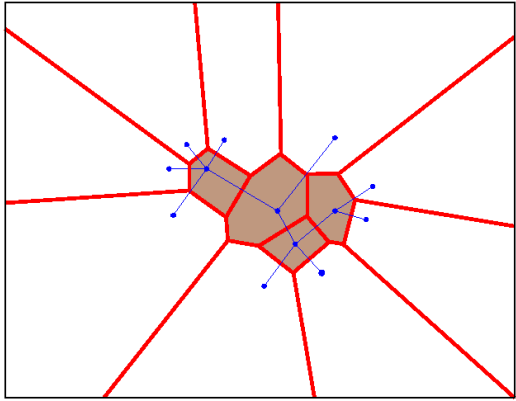
\includegraphics[scale=0.4]{voronoi.png} 
\captionof{figure}{Frontier nodes have a Voronoi region bounded by the space limits. On the contrary, the Voronoi region of nonfrontier nodes is bounded by the Voronoi region of other nodes \cite{jaillet2010sampling}. RRTs naturally balance between exploration and exploitation.}
\end{center}
\end{frame}

\begin{frame}{RRT core modules}
\justify
As stated earlier RRTs are widely used in robotics, but they can be adapted to other areas if the following functions are modified.
\begin{alertblock}{Core modules:}
\begin{itemize}
\item \textbf{Sampling} \\ 
strong relation on how the search space will be explored (i.e. bias toward unexplored regions or a goal state)
\item \textbf{Estimating the nearest neighbor} \\
proximity evaluation of the tree nodes and a sampled state (usually measured by Euclidean distance)
\item \textbf{Extending the tree} \\
selection of a new node to be added that doesn't violate any constraints 
\end{itemize}
\end{alertblock}
\end{frame}

\section{Paper - Adapting a RRT for AP} % change section name to Rapidly-Exploring Planning Tree

\begin{frame}{Motivation}
Motion planning is an area closely related to automated planning \cite{alcazar2011adapting}
\vspace{0.5cm}

RRTs may be able to overcome some of the shortcomings that forward search planners have while keeping most of their desired properties.

\vspace{0.5cm}
Employ RRTs focused on satisficing planning problems.
\begin{alertblock}{Advantages of RRT for Automated Planning:}
\begin{itemize}
\item good balance between exploitation and exploration during search
\item bounded local searches (minimizing exploration of $h$ plateaus)
\item relatively small memory footprint
\item broad range of techniques during local searches
\end{itemize}
\end{alertblock}
\end{frame}

\begin{frame}{Objective}
Adapt RRTs to propositional planning domains, with the following formulation: $P=(S,A,I,G)$

Where:
\begin{itemize}
\item \textbf{S} is a set of atomic propositons; 
\item \textbf{A} is the set of grounded actions derived from the operators of the domain;
\item \textbf{I} is the initial state;
\item \textbf{G} is the set of goal propositions
\end{itemize}
\end{frame}

\begin{frame}{Contributions from previous work}
\begin{exampleblock}{RRTs in discrete search spaces\cite{morgan2004sampling}}
Adapting RRTs to grid worlds and similar classical search problems
\vspace{0.5cm}
\begin{table}[H]
\begin{flushleft}
\caption{RRT modifications for discrete space}
\vspace{-0.5cm}
\begin{tabular}{|l|l|}
\hline
\rowcolor[HTML]{34696D} 
{\color[HTML]{000000} \textbf{RRT module}} & {\color[HTML]{000000} \textbf{Employed technique}}        \\ \hline
Sampling                                   & randomly sample a state that it's not already in the tree \\ \hline
Nearest Neighbor                           & "ad-hoc" heuristic estimation of the cost of reaching     \\
                                           & the sampled state from a given node of the tree           \\ \hline
Extend                                     & local planner limited by the number of nodes expanded     \\ \hline
\end{tabular}
\end{flushleft}
\end{table}
\end{exampleblock}
\end{frame}

\begin{frame}{Contributions from previous work}
\begin{exampleblock}{RRT-Plan\cite{burfoot2006rrt}}
Directly related to Automated Planning, was proposed as a stochastic planning algorithm inspired by RRTs for deterministic planning tasks.

% Please add the following required packages to your document preamble:
% \usepackage[table,xcdraw]{xcolor}
% If you use beamer only pass "xcolor=table" option, i.e. \documentclass[xcolor=table]{beamer}
\begin{table}[]
\centering
\caption{RRT modifications for classical planning}
\vspace{-0.5cm}
\begin{tabular}{|l|l|}
\hline
\rowcolor[HTML]{34696D} 
{\color[HTML]{000000} \textbf{RRT module}} & {\color[HTML]{000000} \textbf{Employed technique}}      \\ \hline
Sampling                                   & sample from a subset of propositions from the goal      \\ \hline
Nearest Neighbor                           & caches the cost of achieving every goal proposition     \\
                                           & from a state                                            \\ \hline
Extend                                     & local planner limited by the number of nodes expanded   \\ \hline
\end{tabular}
% \begin{tabular}{|l|l|} -- como eu estava entendendo o nearest neighbor
% \hline
% \rowcolor[HTML]{34696D} 
% {\color[HTML]{000000} \textbf{RRT module}} & {\color[HTML]{000000} \textbf{Employed technique}}      \\ \hline
% Sampling                                   & sample from a subset of propositions from the goal      \\ \hline
% Nearest Neighbor                           & caches the cost of achieving every atom in the state    \\
%                                            & using $h^+$ heuristic, so the nearest neighbor will be: \\
%                                            & $ argmin \sum_{p \in sample} h^+(p)$                    \\ \hline
% Extend                                     & local planner limited by the number of nodes expanded   \\ \hline
% \end{tabular}
\end{table}
\end{exampleblock}
\end{frame}

% \begin{frame}{Proposed improvements}
% \begin{alertblock}{Proposed work:}
% \begin{itemize}
% \item sample the implicit search space more uniformly
% \item 
% \end{itemize}
% \end{alertblock}
% \end{frame}

\begin{frame}{Random Planning Tree (RPT)}
\justify
\textbf{\large\alert{SAMPLING}}\\[0.3cm]
Uniform sampling of the search space using \alert{state invariants as constraints}. Sampling is perform by choosing propositions from each invariant group such that is not in mutex with any other selected proposition for $q_{rand}$.

For every sampled state a reachability of goals is performed, if some goal proposition is unreachable, the state is discarded.

\textbf{``exactly-1" invariant group} - set of propositions that only one can be true in a state at the same time.

\textbf{$h^2$ heuristic} - approximate the cost of a set of atoms by the cost of the most costly atom \textit{pair} in the set. A pair with infinite cost is a binary mutex, implying that they can't belong to the same state. 
\end{frame}

\begin{frame}{Random Planning Tree (RPT)}
\justify
\textbf{\large\alert{NEAREST NEIGHBOR}}\\[0.3cm]
Finding the closest node of the tree to a sampled state $q_{rand}$ requires a distance estimation. In Automated Planning, this measurement is evaluated using heuristics derived from reachability analysis, like $h^{add}$ and $h^{ff}$.

Since each extend phase of RRT requires a distance evaluation, estimating the cost to every sample state can make the problem intractable. 

RPT caches the \textit{best support} action (first action to achieve a proposition) for every proposition in the state. 

-- esperar resposta do email para detalhar mais o funcionamento dessa parte do hff --
% in this case, the closest node is the one wiht the lowest cost (# of actions) of achieving every proposition in the sampled state initiating from cached best supported actions%
\end{frame}

\begin{frame}{Random Planning Tree (RPT)}
\justify
\textbf{\large\alert{EXTEND}}\\[0.3cm]
Tree is built from the initial state and node contains a state, a link to its parent, a plan that leads from its parent to the state and the cached best supporters for every proposition.

There is a probability $p$ of advancing towards the goal and a probability $1-p$ of advancing towards a sampled state.

Local search limited by an $\varepsilon$ number of nodes can be performed at most two times per iteration: 

\hspace{0.5cm}
- if with a probability $p$, tries to extend toward a sampled state, returning  $q_{new}$ as the closest node of this local search 

\hspace{0.5cm}
- another one to find a promising node $q_{new_{goal}}$ towards the goal

After every local search, a new node is added to the tree.
\end{frame}

% \begin{frame}{Comparison and results}

% \end{frame}

\section{References}
% [allowframebreaks] múltiplos slides de referências
\begin{frame}[allowframebreaks]{References}
  \bibliography{my_references}
  \bibliographystyle{abbrv}
\end{frame}

\end{document}